\section{Deliberate Score Grouping}
\label{sec-roundingoff}

We now consider whether the deliberate use of tied scores -- which
might allow efficiency improvements in the underlying search system
-- has a discernible effect on retrieval effectiveness.

\myparagraph{Score Approximation}

Scoring documents using modern similarity computations involves
non-trivial amounts of arithmetic, especially if phrase components or
term proximity components are being used.
Regimes such as WAND {\citep{bchsz03cikm}} seek to minimize the
number of documents scored, while still giving rise to exactly the
same ranking for the top-$k$ documents, an approach that meets the
requirements for being {\emph{rank safe to depth $k$}}.
That is, the WAND process ensures that all of the documents in the
first $k$ positions of the ranking are in their ``right'' positions
in the ranking that is generated, but makes no such guarantee for
documents beyond depth $k$.
This is a relatively stringent requirement, and other
computation-pruning techniques might also be considered that provide
alternative and more flexible trade-offs.

In particular, we now consider the following weaker requirement: that
each document must be scored in a manner that guarantees that it is
in the correct {\emph{band}} of the ranking, where the bands are
defined geometrically based on a parameter $\rho>1$.
More precisely, let $b_1=1$, and thereafter let
$b_{g+1}=\lceil{\rho\cdot b_g}\rceil$.
The $g$\,th group, for $g\ge1$, spans the ranks from $b_g$ to
$e_g=b_{g+1}-1$ inclusive.
For example, if $\rho=2$, then the bands are $[1\ldots1]$,
$[2\ldots3]$, $[4\ldots7]$, and so on; and if (say) $\rho=1.62$ (the
golden ratio) the bands are $[1\ldots1]$, $[2\ldots3]$, $[4\ldots6]$,
$[7\ldots11]$, and so on, with widths given by the Fibonacci
sequence.
The smaller the value of $\rho$, the smaller each of the groups is,
and the closer the approximate ranking is to the ``true'' and exact
ranking.
As $\rho$ approaches $1$, the retrieval system is obliged to place
each of the documents closer and closer to its final ``correct''
position, without regard for $k$, the run length.
That is, for a given value of $\rho$, we allow the retrieval system
to economize on its computational costs and return bands of documents
$[b_g\ldots e_g]$, with equal scores assumed within each band.

\myparagraph{Worst-Case Bounds}

\alistair{For RR and RBP can compute upper bounds on the difference
difference in score that is possible, as a function of
$\rho$. Maybe can also say something about AP too, who knows.}

\myparagraph{Effectiveness Score Changes}

Given these upper bounds, it is appropriate to ask: to what extent
does an allowance for rank-based score imprecision affect retrieval
effectiveness in practice?
To respond to this question, we make use of TREC resources, taking
the same system runs as were already examined in
Section~\ref{sec-trecimpact}, and in effect mapping all of the
documents ranked in band $g$ to a synthetic score of $1/g$, as if the
retrieval system had deliberately not carried out the extra
computation that would be needed to fully differentiate between the
approximately $\rho^g$ documents in that band.

\begin{figure}[t!]
\centering
\subfloat[RR\label{fig-score-variation-rr}]{%
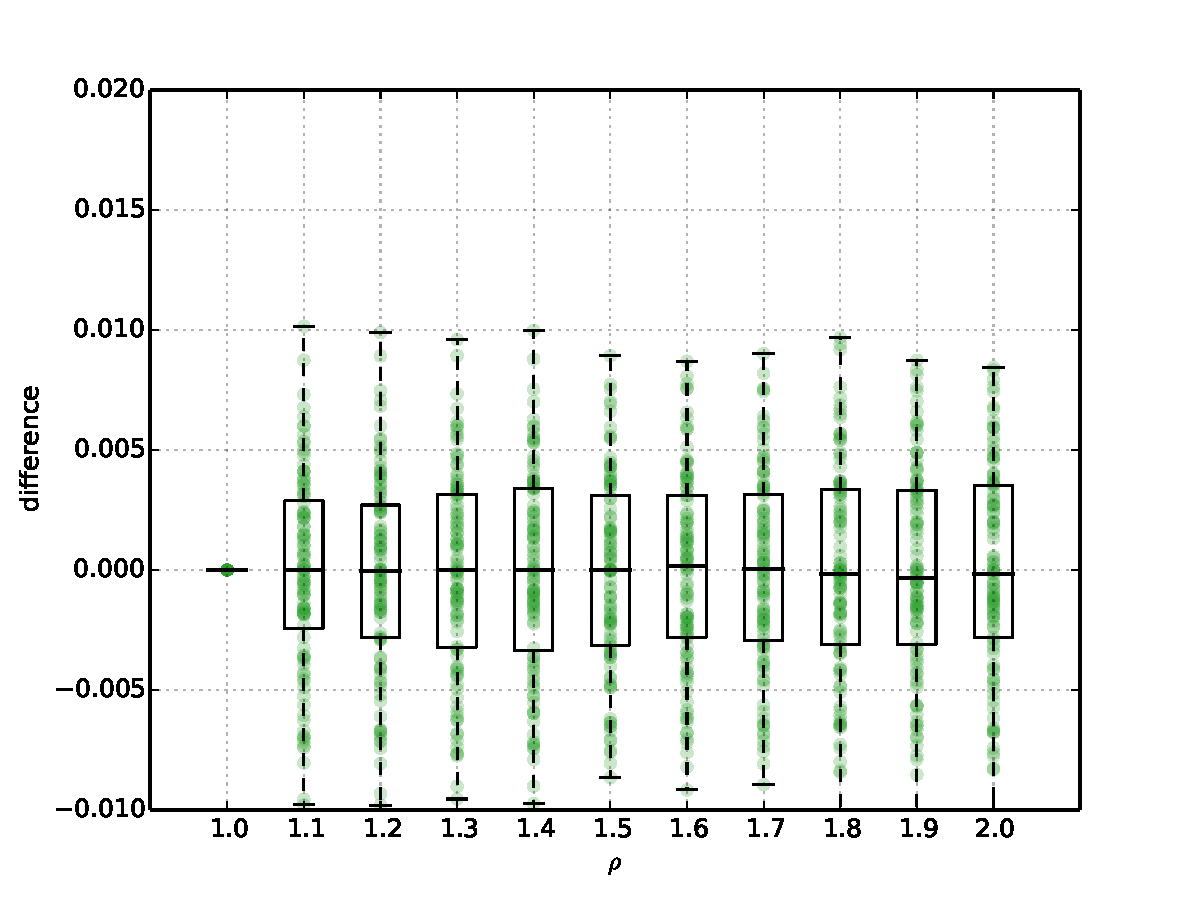
\includegraphics[width=0.49\textwidth]{figs/rho_diff_RR_scaled.pdf}
}
\subfloat[RBP0.6\label{fig-score-variation-rbp50}]{%
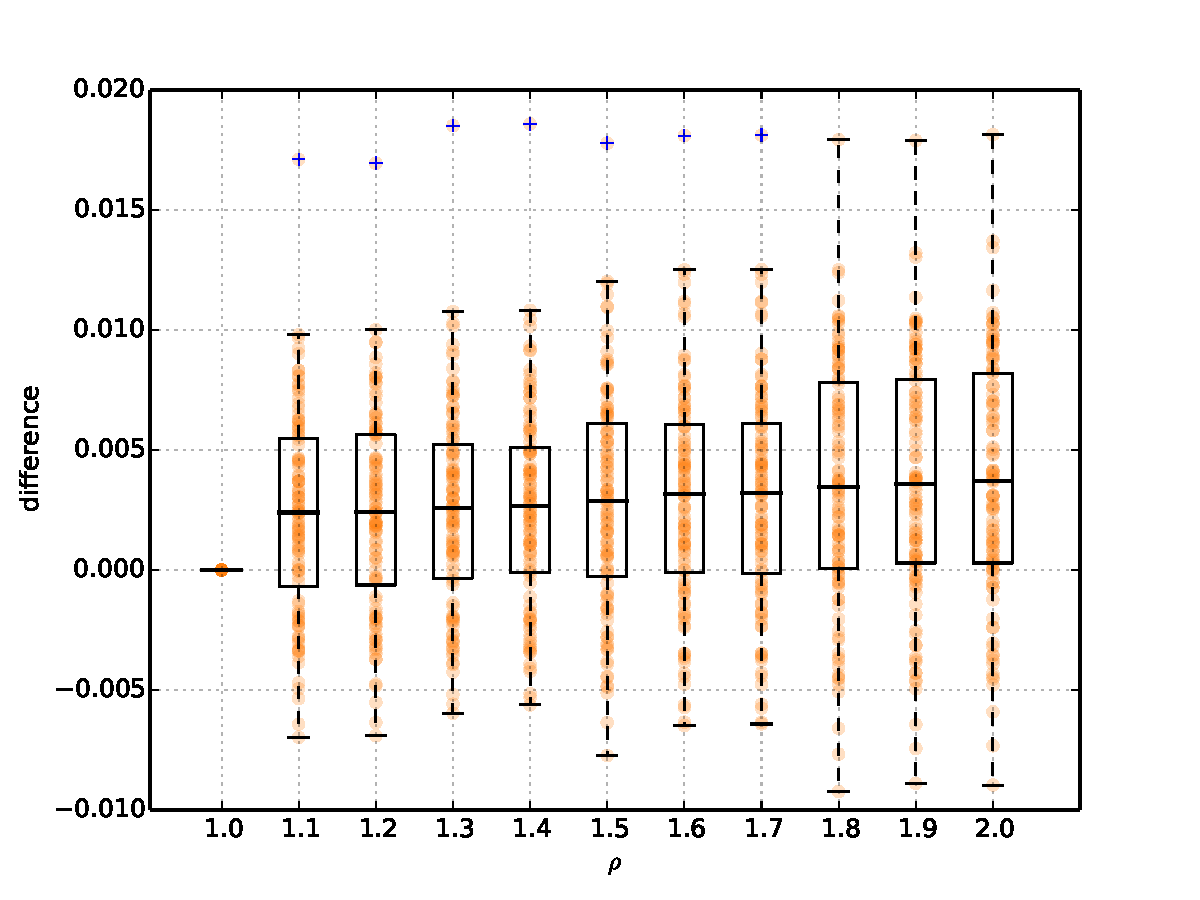
\includegraphics[width=0.49\textwidth]{figs/rho_diff_RBP06.pdf}
}
\\
\subfloat[RBP0.85\label{fig-score-variation-rbp85}]{%
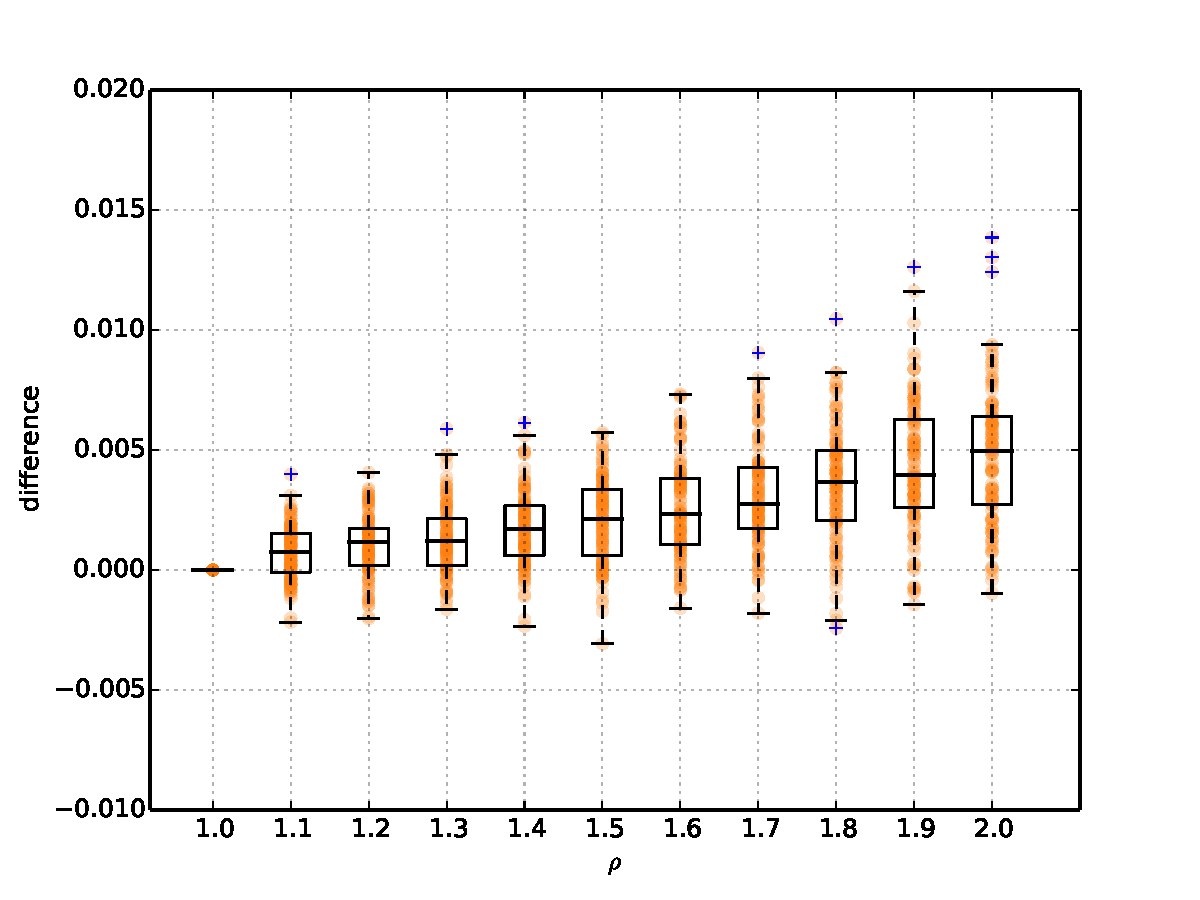
\includegraphics[width=0.49\textwidth]{figs/rho_diff_RBP085.pdf}
}
\subfloat[AP\label{fig-score-variation-ap}]{%
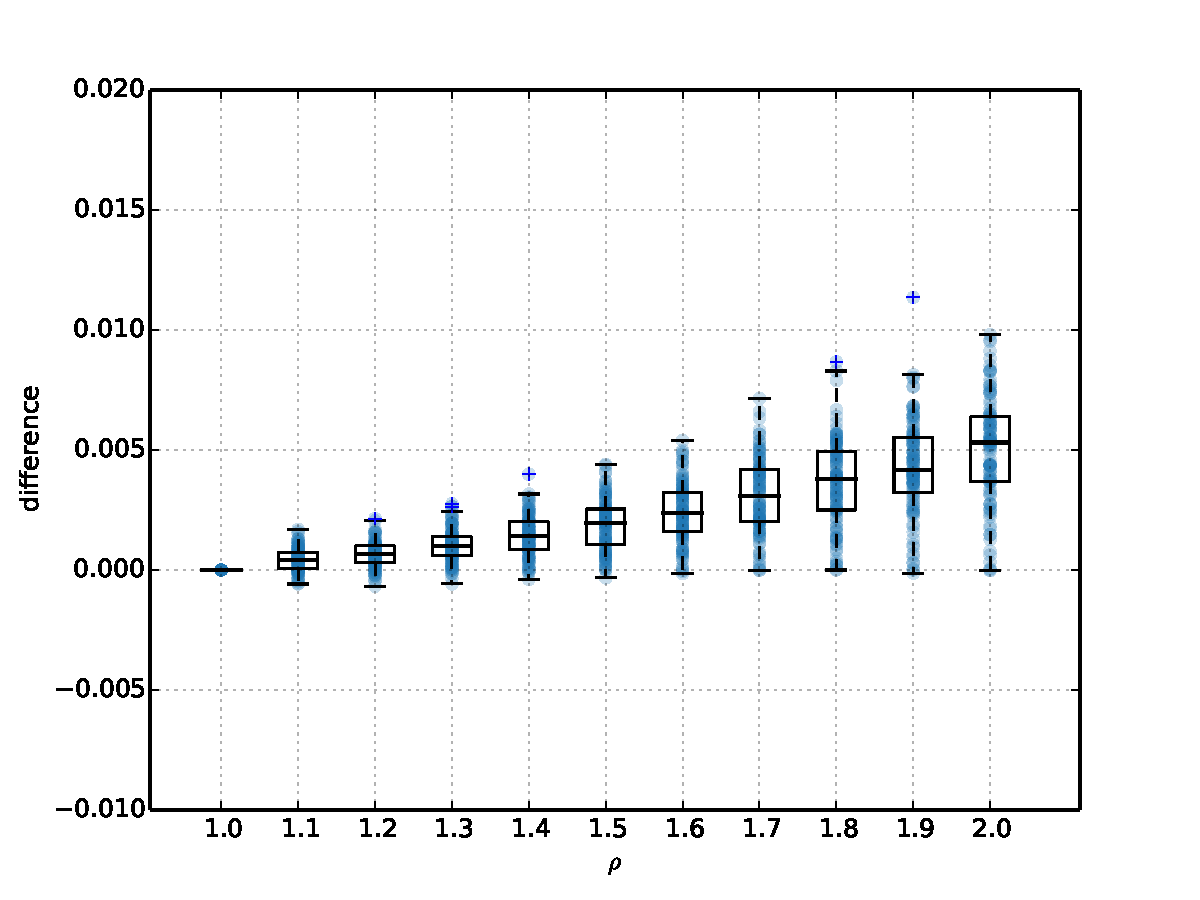
\includegraphics[width=0.49\textwidth]{figs/rho_diff_AP.pdf}
}
\caption{Variation in metric effectiveness score across a set of $103$
runs and $50$ topics ($103$ points plotted in total in each column), as a
function of $\rho$, for four different retrieval effectiveness
metrics.
\alistair{Why not $50\times 103$ points in each column? Why only $103$?}
\alistair{Something seems incorrect in the RBP0.60 graph.
Why the sudden jump at the start?}
\alistair{Change from RBP0.6 to RBP0.5.}
\alistair{Fonts on axis labels need to be larger.}
\label{fig-score-variation}}
\end{figure}

Our first experiment explores the score variance introduced as a
result of score ``banding'', calculating for a set of runs from the
1998 TREC7 experimentation the variation in run score that results
when a given degree of score imprecision is introduced.
In all cases the score difference calculated is the
across-permutations computation that was illustrated in
Section~\ref{sec-ties} when applied to the deliberately-tied
rankings, compared to the score the same metric achieves on the
original submitted ranking for that same topic.
(We used our own version of {\tt{trec\_eval}} to ensure that this was
done consistently.)
We followed standard protocols and assumed that unjudged documents
were not relevant for the purposes of scoring the runs.

Figure~\ref{fig-score-variation} shows the results of this
{\alistair{Build the graph, and then discuss what it shows.
Hopefully it shows something interesting or at least a little bit
unexpected.}}

\begin{figure}[t!]
\centering
\subfloat[RR\label{fig-rho-p-value-rr}]{%
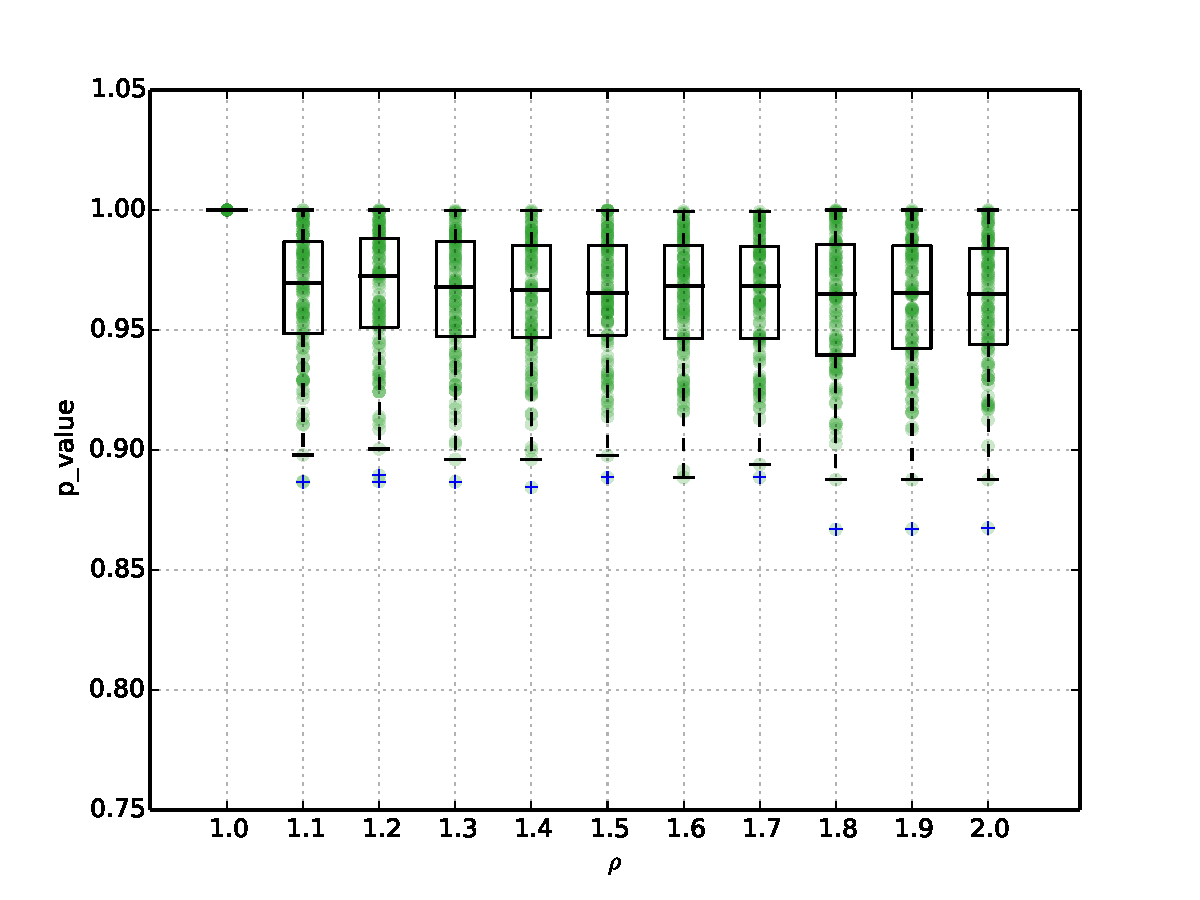
\includegraphics[width=0.49\textwidth]{figs/rho_pvalue_RR.pdf}
}
\subfloat[RBP0.6\label{fig-rho-p-value-rbp50}]{%
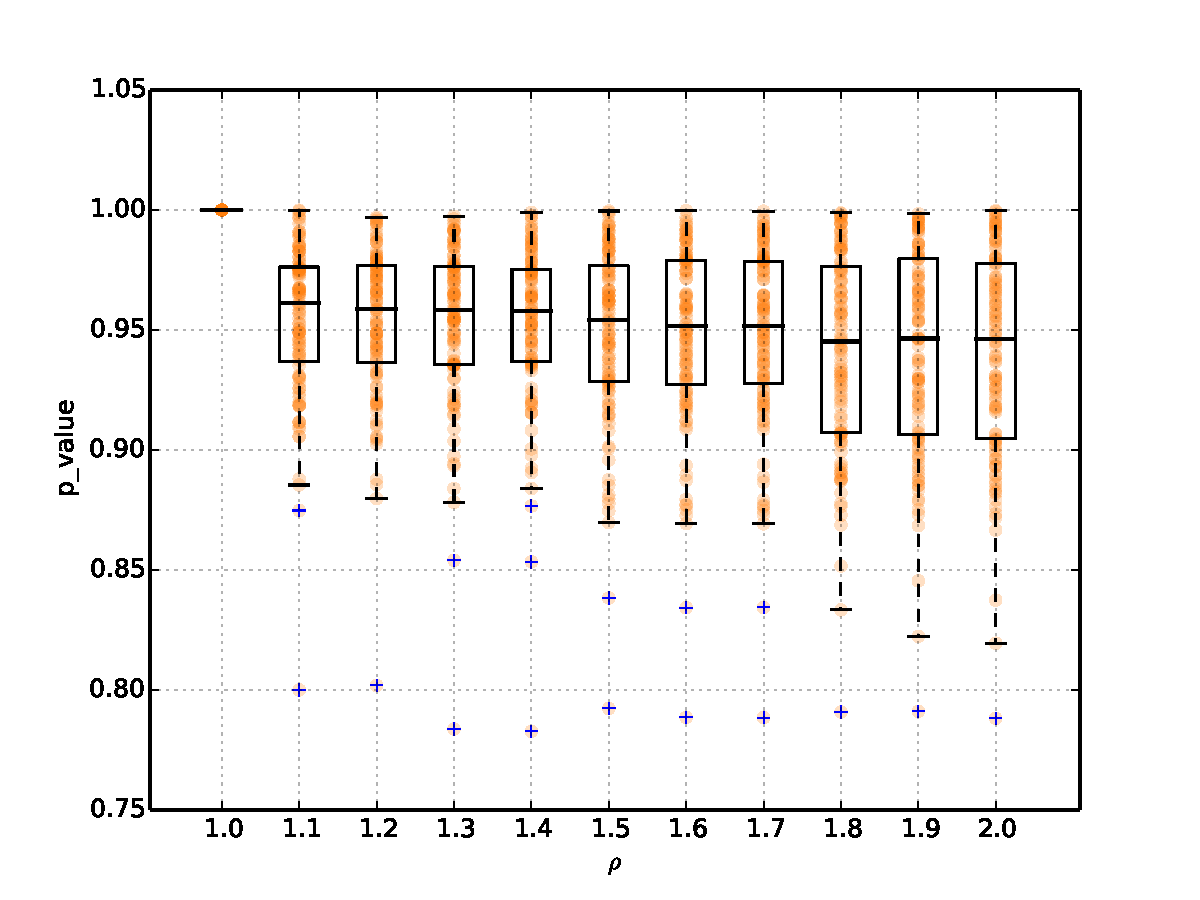
\includegraphics[width=0.49\textwidth]{figs/rho_pvalue_RBP06.pdf}
}
\\
\subfloat[RBP0.85\label{fig-rho-p-value-rbp85}]{%
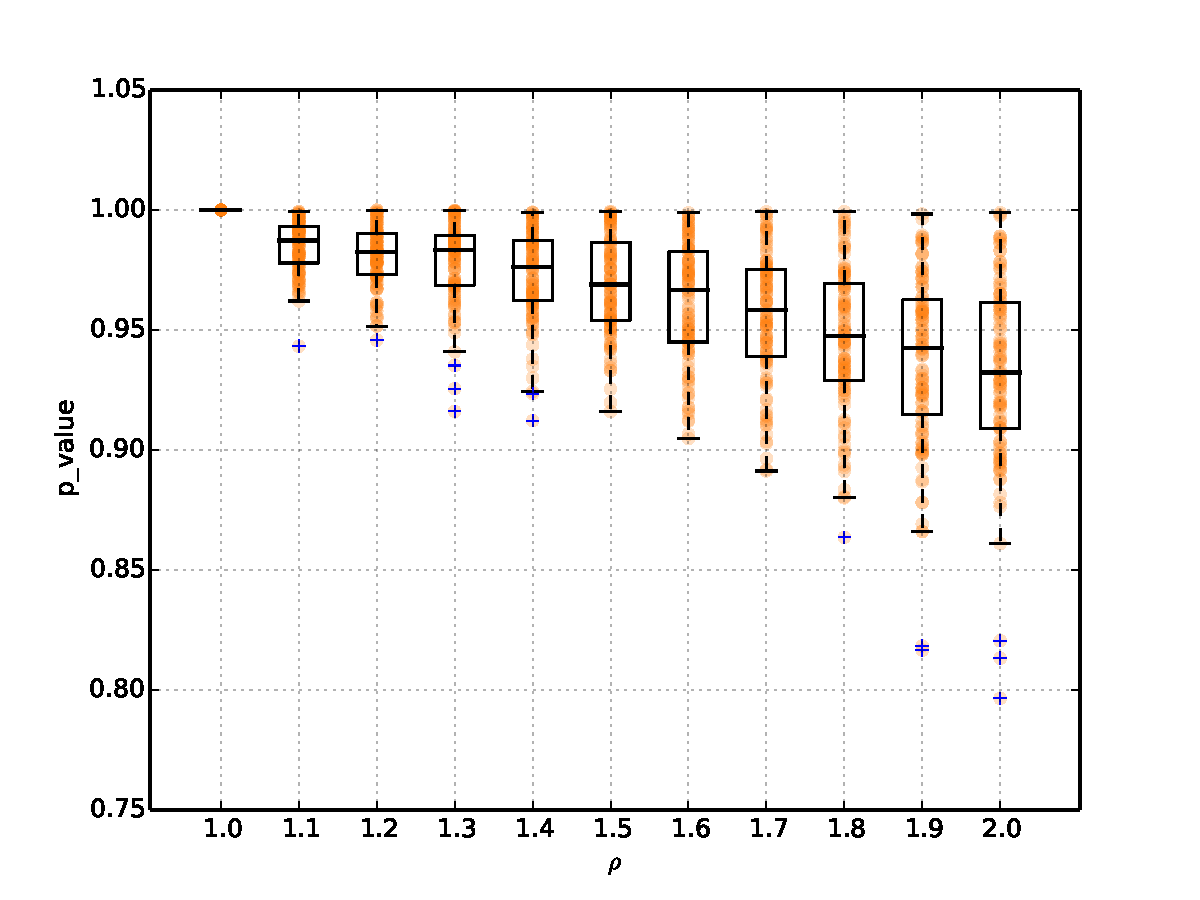
\includegraphics[width=0.49\textwidth]{figs/rho_pvalue_RBP085.pdf}
}
\subfloat[AP\label{fig-rho-p-value-ap}]{%
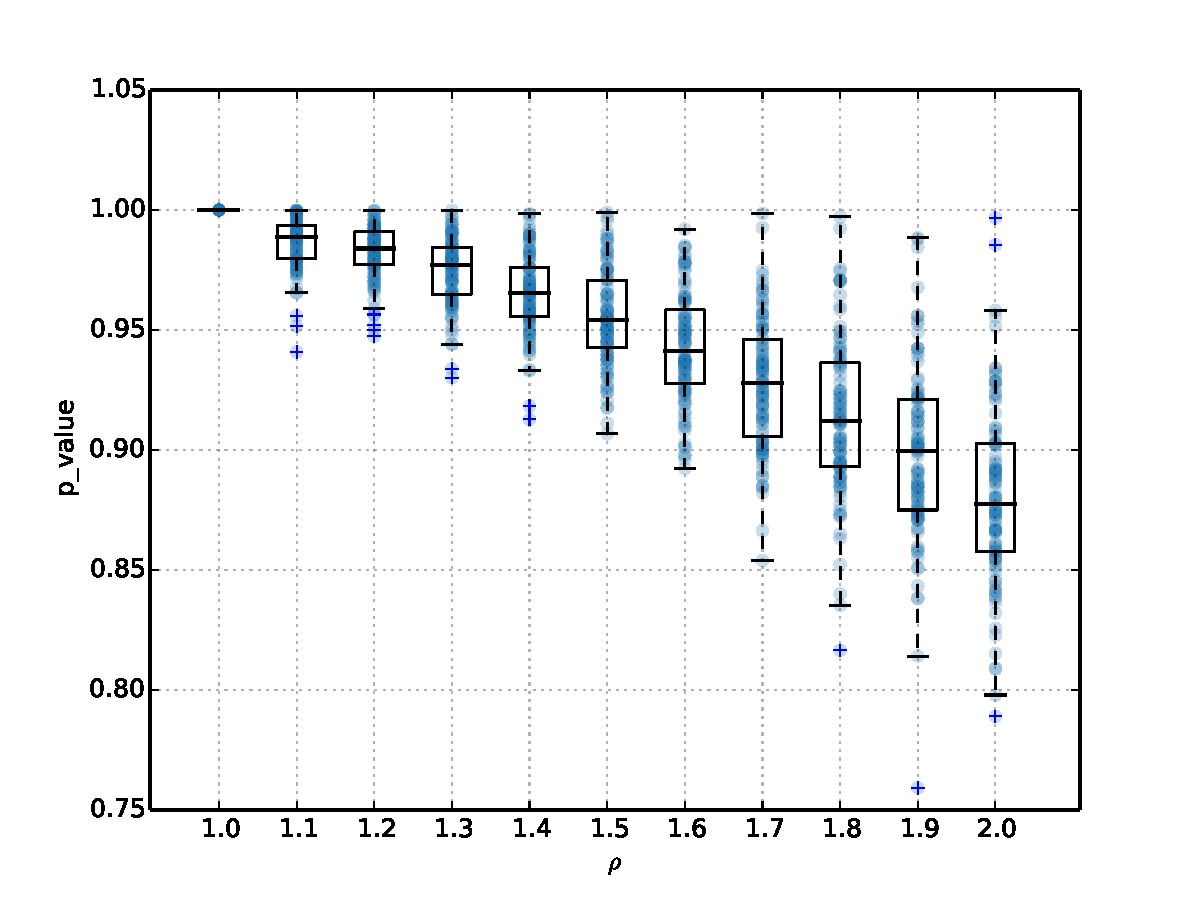
\includegraphics[width=0.49\textwidth]{figs/rho_pvalue_AP.pdf}
}
\caption{Student $t$-test values when comparing system scores for
$103$ original-order runs, and the corresponding set of $103$
grouped-score runs ($103$ points plotted in each column).
A $p$ value of $1.0$ indicates that the two systems yield identical
outcomes across the $50$ topics.
\alistair{Something still incorrect in the RBP0.60 graph?
Or does the jump at the start now reflect what is happening with RR?
Check everything!}
\alistair{Change from RBP0.6 to RBP0.5.}
\alistair{Fonts on axis labels need to be larger.}
\label{fig-rho-p-value}}
\end{figure}

\myparagraph{System Comparison Sensitivity}

Effectiveness measurements are also used to compare systems in a
pairwise manner.
In the second experiment, we explore the implications that score
rounding has on the ability of metrics to differentiate between
systems.
The normal approach to comparing systems is to take their computed
scores across a set of topics, and perform a paired $t$-test to
explore the null hypothesis that the two systems are in fact the
same.
The process of carrying out the $t$-test generates a $p$ value; the
smaller the $p$ value, the smaller the chance that the two systems
being compared are giving the same performance.
To establish significance, a threshold value $\alpha$ is employed,
often $\alpha=0.05$, with $p\le\alpha$ being regarded as a
significant outcome.

\begin{figure}[t]
\centering
\rule{0.5mm}{45mm}
\caption{Variation in $p$ values across system pairs in a set
of runs, plotted as a function of $\rho$, for three different
retrieval effectiveness metrics.
{\alistair{RR, RBP0.85, AP?}}
{\alistair{$\rho = 1.0, 1.1, 1.2, 1.3, \ldots, 2.0$, or something like
that.}}
{\alistair{Box and whisker plot, as $\rho$ is smaller, the mean score
difference should get closer to zero, and the variance should also be
getting smaller.
RR should be relatively unaffected, the others will have broader
variance.
Would be cool in the mean stayed near zero even when $\rho$ is
relatively large.}}
{\alicia{I am sure what should be placed here... have not they all been placed in Figure 2? }}
\label{fig-pair-variation}}
\end{figure}

To measure the effect that score rounding has on system comparisons,
we took the 50 topics of the TREC7 {\todo{citation}} collection
and the 103 runs associated with it, and computed: (a) a set
of $p$ values, generated by comparing each pair of systems using the
metric scores associated with the original set of runs; and then (b)
the corresponding set of $p$ values, generated when the same runs are
first mapped into group scores, and the all-permutations averaging
technique applied.

\myparagraph{Results}
